% 
% Annual Cognitive Science Conference
% Sample LaTeX Paper -- Proceedings Format
% 

% Original : Ashwin Ram (ashwin@cc.gatech.edu)       04/01/1994
% Modified : Johanna Moore (jmoore@cs.pitt.edu)      03/17/1995
% Modified : David Noelle (noelle@ucsd.edu)          03/15/1996
% Modified : Pat Langley (langley@cs.stanford.edu)   01/26/1997
% Latex2e corrections by Ramin Charles Nakisa        01/28/1997 
% Modified : Tina Eliassi-Rad (eliassi@cs.wisc.edu)  01/31/1998
% Modified : Trisha Yannuzzi (trisha@ircs.upenn.edu) 12/28/1999 (in process)
% Modified : Mary Ellen Foster (M.E.Foster@ed.ac.uk) 12/11/2000
% Modified : Ken Forbus                              01/23/2004
% Modified : Eli M. Silk (esilk@pitt.edu)            05/24/2005
% Modified : Niels Taatgen (taatgen@cmu.edu)         10/24/2006
% Modified : David Noelle (dnoelle@ucmerced.edu)     11/19/2014

%% Change "letterpaper" in the following line to "a4paper" if you must.

\documentclass[10pt,letterpaper]{article}

\usepackage{cogsci}
\usepackage{pslatex}
\usepackage{apacite}
\usepackage[caption=false,font=footnotesize]{subfig}

\usepackage{tikz}
\usetikzlibrary{arrows,shapes,backgrounds,petri,fit}




\title{Curiosity-Driven Development of Tool Use Precursors: a Robotic Model}
 
\author{{\large \bf S\'ebastien Forestier (sebastien.forestier@inria.fr)} \\
	Inria Bordeaux Sud-Ouest and Ensta Paristech, France
  \AND {\large \bf Pierre-Yves Oudeyer (pierre-yves.oudeyer@inria.fr)} \\
	Inria Bordeaux Sud-Ouest and Ensta Paristech, France}


\begin{document}

\maketitle


\begin{abstract}
This is the abstract.

\textbf{Keywords:} 
curiosity-driven learning; tool use; goal babbling; overlapping waves; developmental trajectory; hierarchical skill learning; HiCu model
\end{abstract}


\section{Introduction}

	
	The understanding of tool use development in young children is one of the key question for the more general understanding of the ontogeny of human cognition.
	Indeed, a series of abilities are progressively developed from the simplest reaching movements of the arms through more dexterous manipulation of a spoon, towards advanced control of multiple interacting objects.
	The latter shows an understanding of shapes, forces and other physical properties that can be recruited for mental transformations and planning operations which are pillars of human cognition.
	Children's development has first been described as staircase-like successive stages in which all children go through \cite{piaget1952origins}.
	More recently, a different view was developed \cite{siegler1996emerging} describing variability among children's developmental paths and in a child's set of current methods to solve a same task. 
	This applies in particular to the development of tool use precursors, which can be described as three consecutive and overlapping stages of behaviours \cite{guerin2013survey}: 
	behaviours without objects, behaviours with a single object, and behaviours with several interacting objects.
	A study of free play \cite{Zelazo198095} shows that at $9\frac{1}{2}$ months play is mostly composed of tactile examination, waving, banging and mouthing of a single object, 
	but that simple relational acts of banging two objects together is already common.
	Later at $13\frac{1}{2}$ months, the study reveals that most children instead prefer to explore the relationships
	among objects, but still show behaviors of the previous phase. 
	Furthermore, they show that this overlapping phases pattern averaged across children is also present in a longitudinal study of a single child.
	
	In this paper we focus on the study of this seamless progression between overlapping phases of behaviour with objects.	
	We hypothesize that several mechanisms play a role in the structure of this behavioural progression and in particular 
	1) the intrinsic motivation to explore as a self-regulation of the learning growth of complexity, and 
	2) the structure of the representation used to encode sensorimotor experience.	
	Indeed, curiosity-driven learning models with an intrinsic motivation towards situations yielding a high learning progress 
	have shown that developmental trajectories could emerge from the active learning of sensorimotor mappings, in very different settings.
	In the Playground Experiment \cite{oudeyer_what_2007}, a quadruped robot learned how to use its motor primitives to interact with the items of an infant play mat and a robot peer.
	Also, in a study of the self-organization of vocalizations \cite{moulin-frier_self-organization_2014}, an agent had to learn how to
	use a vocal synthesizer by self-exploration or with the help of humans' demonstrations of phonetic items. 
	Their model reproduces accurately major phases of infant vocal development until $6$ month old.
	In both studies, developmental trajectories of increasing complexity are emerging from learning, with both regularities in developmental steps and diversity.
	The diversity comes from different mechanisms: stochasticity in the algorithms, variability in the environment, and the multiples attractors of the dynamic learning system.
	In existing models, the agent learns only one mapping that relates a motor space to a sensory or task space. 
	However, in the perspective of an open-ended development of reusable skills, and specifically in the development of tool use, multiple interdependent and hierarchically organized task spaces should be available to the agent
	as for instance complex actions with tools could make use of previously learned parameterized interaction with the tool.
	
	We study aspects of those hypothesis leveraging previous models of curiosity-driven learning and extending them to the active exploration of sensorimotor and task spaces.
	We define hierarchies of sensorimotor models that structure the sensory space to reflect the interaction of the different items of the environment.
	In such hierarchies of models to explore, different exploration choices are available to the agent at each learning iteration: which model to explore, and how to explore that model.
	The problem of finding an efficient active choice strategy is an instance of strategic learning \cite{nguyen2012}, 
	where different outcomes and strategies are available and the agent has to learn which strategies are useful for which outcomes. 
	We define and compare several strategies to study the role of active learning and hierarchical representation in the structuration of developmental trajectories.
	We compare the different learning conditions in a $2$D environment where a simulated arm with three joints plus a gripper can grab tools to move an out-of-reach object.
	We measure the different phases of behaviour during exploration and compare the structure of the behavioural waves. [more results here?]
	
	Robotics related work.
	\cite{ugur2015}
	To our knowledge, this model is the first to show overlapping waves structure in the development of tool use [can we say it is the first model of curiosity-driven development of tool use ?].
	
	However, here we do not study some other important factors in the development of tool use.
	We consider the hierarchy of models given to the agent and do not study its autonomous building and evolution during developmental stages.
	Also, social guidance with imitation and mimicry is of central importance for the development of tool use in infants but we do not address the question
	of its modeling in this paper nor the interplay and tradeoff between social learning and self-exploration.
	Another important feature of young infants' learning of tool use is the need to adapt to a developing body and to the maturation of vision during ontogenetic development, 
	but here we consider motor control and sensory perception steady over the simulated learning time span.
	
	Footnote
	\cite{forestier2015}
	\cite{unifying}

	Along with this paper we provide open-source Python code\footnote{Source code and notebooks available as a Github repository at \url{https://github.com/sebastien-forestier/CogSci2016}} 
	with iPython/Jupyter notebooks that explain how to reproduce the experiments and analysis. 
	
	%Representations in explauto and other models 
	%\cite{mugan2009}
	%\cite{metzen2013}
	%%\cite{horde}
	%%\cite{mugan}
	%\cite{vig}
	%\cite{sutton1999between}
	
%

\section{Methods}

	\subsection{Environment}
	
		We simulate a 2D robotic arm that can grasp tools that can be used to move an object into different boxes in the environment. 		
		In each trial, the agent executes a motor trajectory, we evaluate its consequences on the sensory dimensions and we give him
		this sensory feedback. Finally the arm, tools and objects are resetted to their intial state.
		The next sections precisely describe the different items of the environment and their interactions.	
		See Fig.\ref{env} for an exemple state of the environment. 
		
		\begin{figure}[h]
			\centering
			\hspace{-0.73cm}
			\vspace{-0.59cm}
			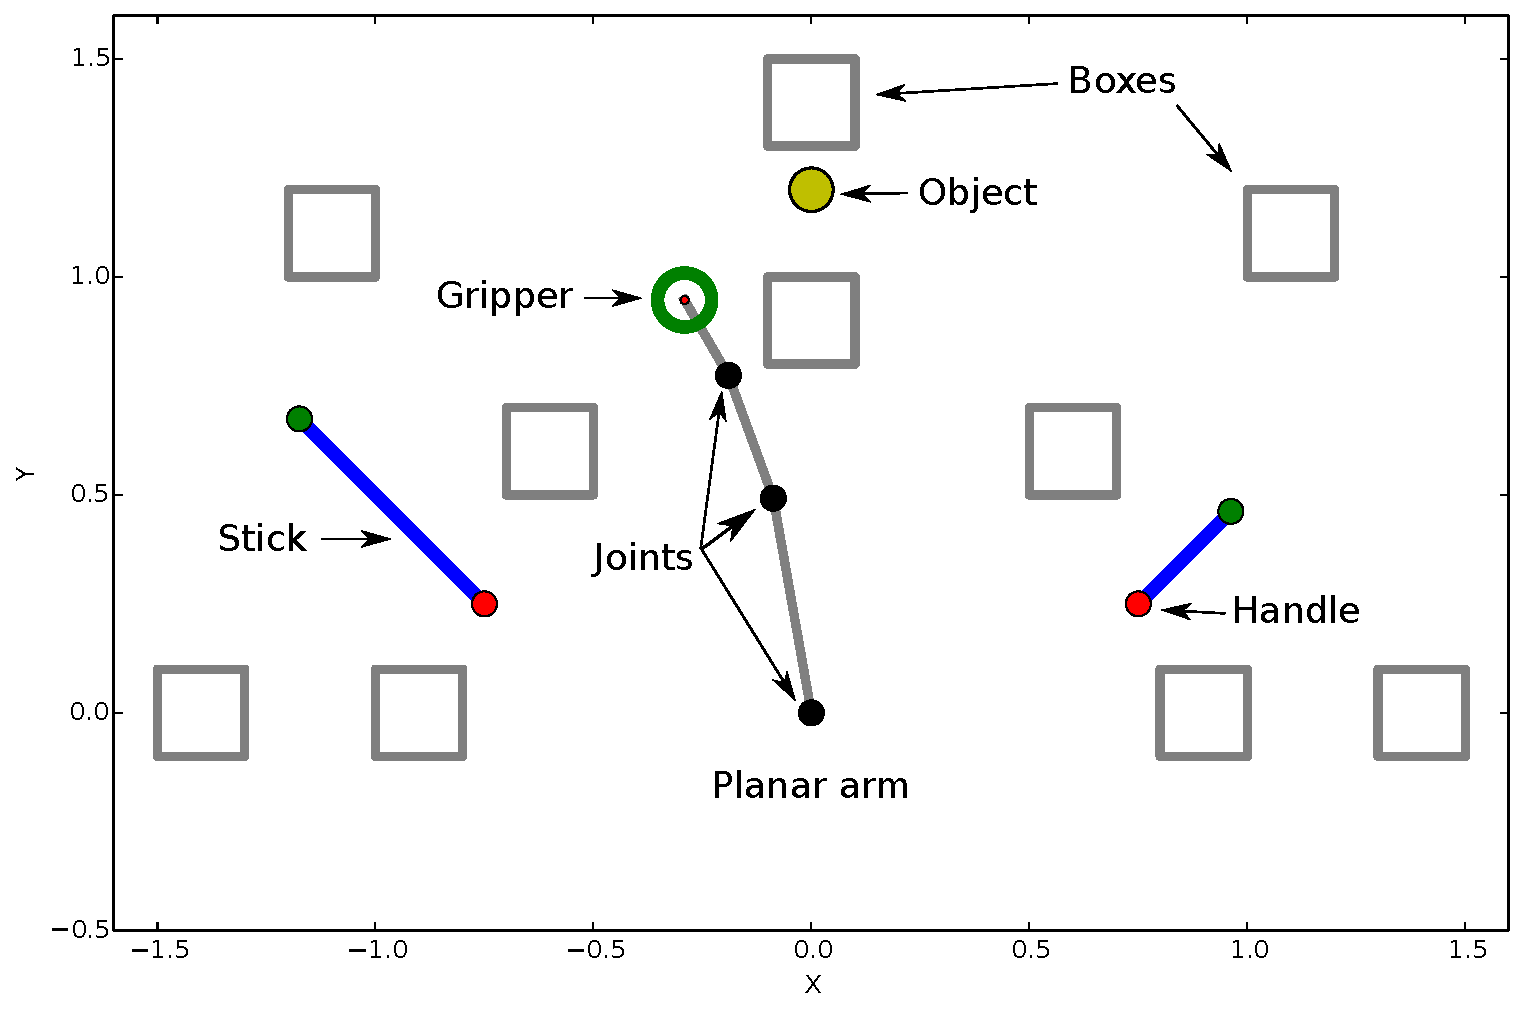
\includegraphics[width=9.12cm]{./include/tools.pdf}
			\subfloat{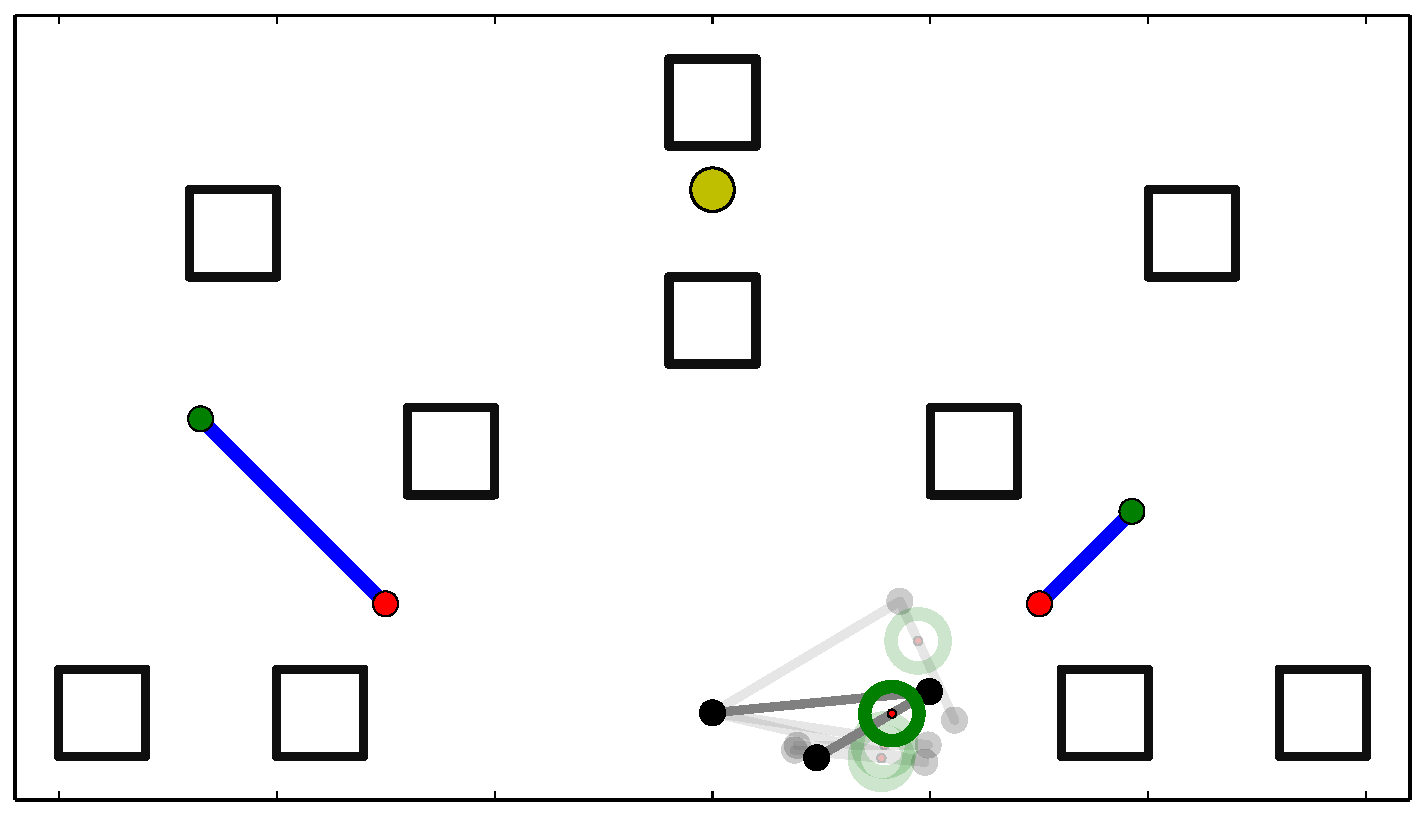
\includegraphics[width=2.8cm]{./include/mvt-16.pdf}}
			\subfloat{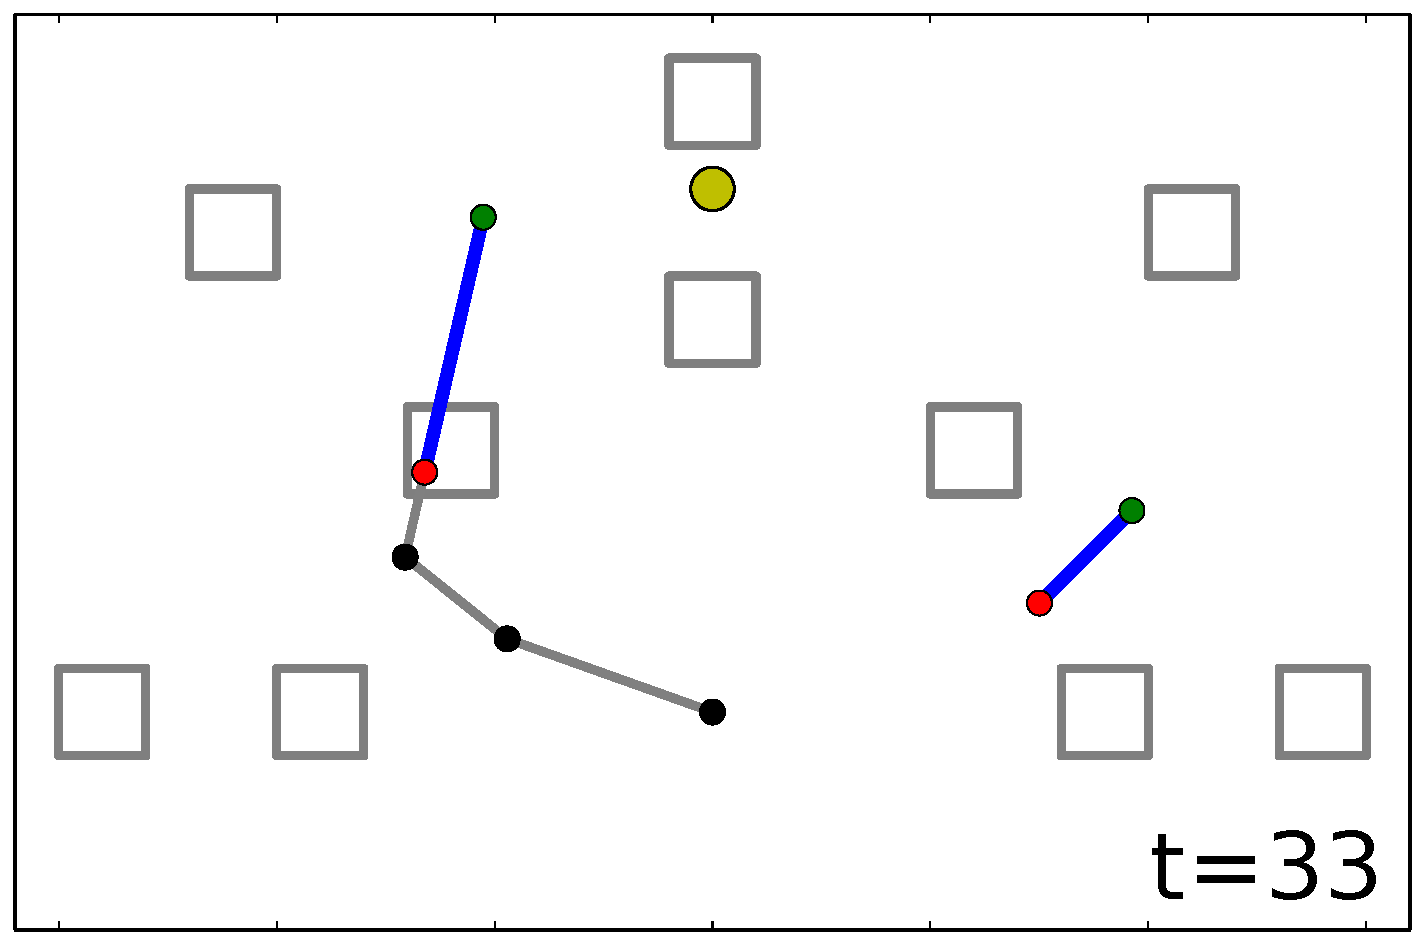
\includegraphics[width=2.8cm]{./include/mvt-32.pdf}}
			\subfloat{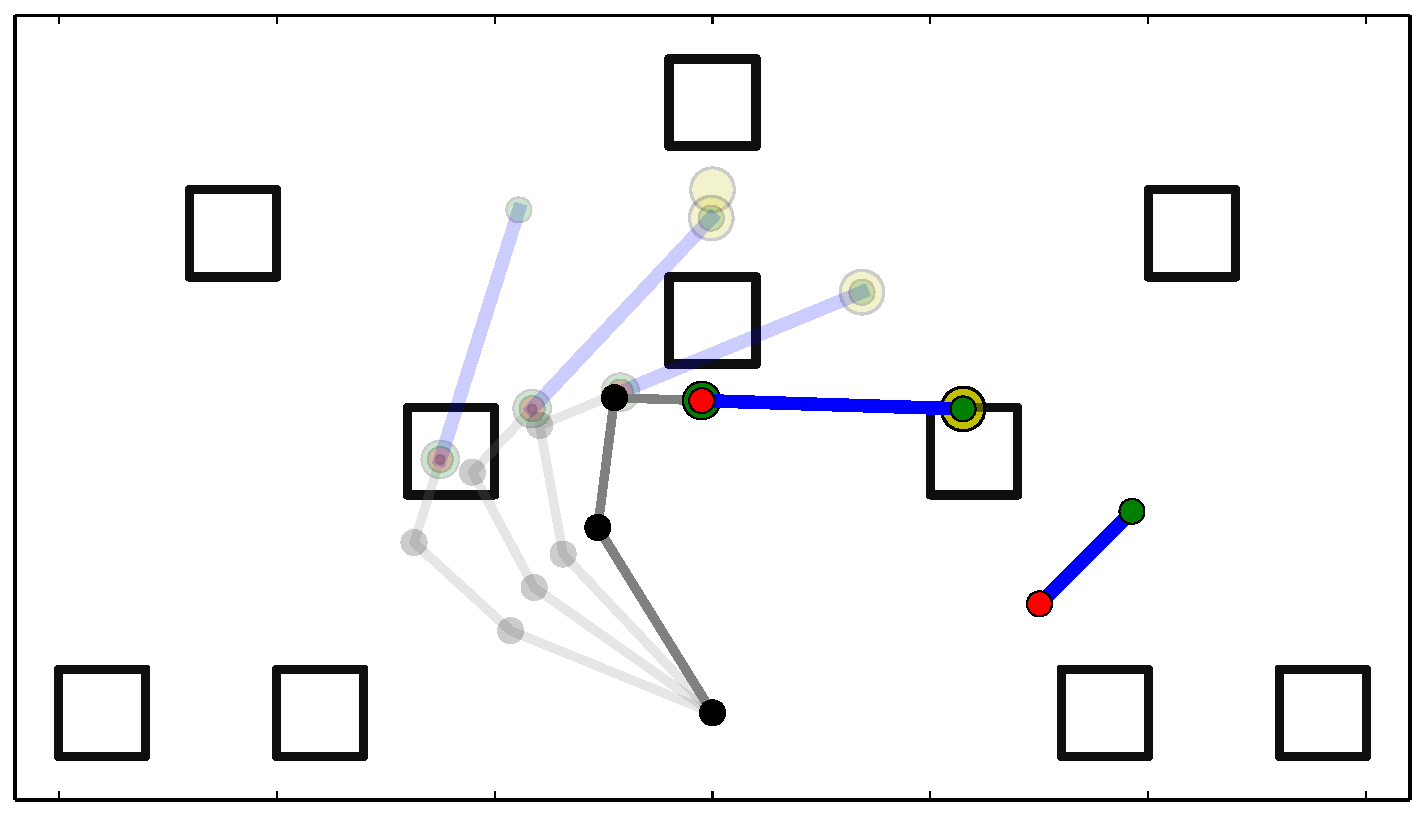
\includegraphics[width=2.8cm]{./include/mvt-49.pdf}}\\
			\hspace{-0.42cm}
			\subfloat{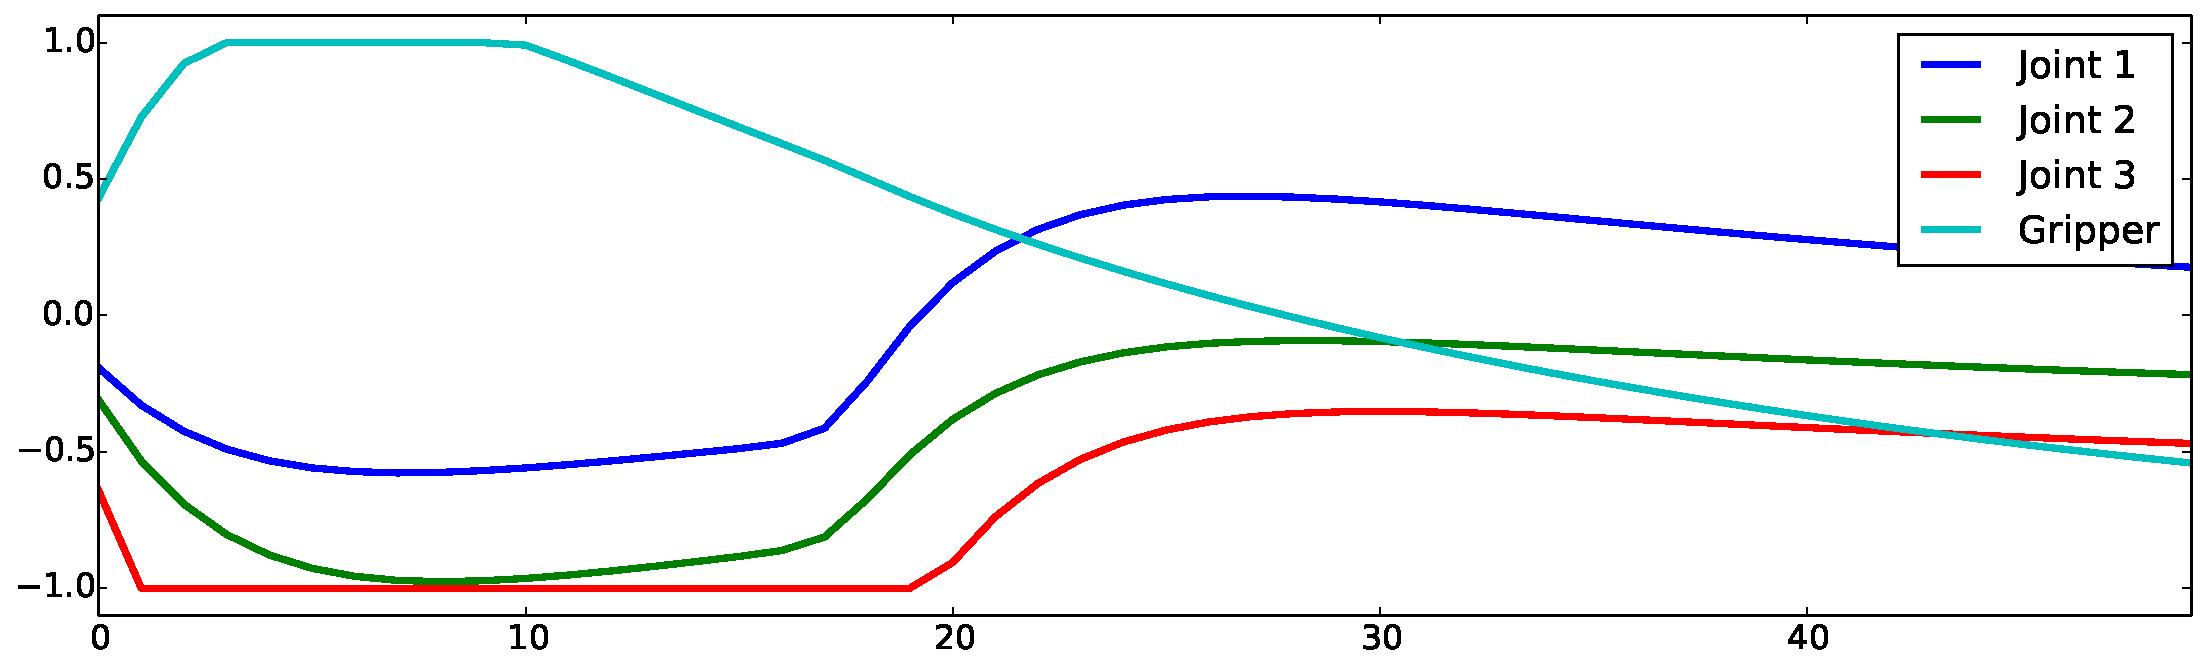
\includegraphics[width=8.8cm]{./include/dmp.pdf}}
			\caption{Top: a state of the environment. Middle: position of the arm at time steps $17$, $33$ and $50$ along the $50$ steps movement. Bottom: trajectory of each of the four virtual motors, generated by a DMP.}
			\label{env}
		\end{figure}

		\subsubsection{Robotic arm}
		
			The 2D robotic arm has $3$ joints plus a gripper located at the end-effector.
			Each joint can rotate from $-\pi~rad$ to $\pi~rad$ around its resting position, mapped to a standard interval of $[-1,1]$.
			The length of the $3$ segments of the arm are $0.5$, $0.3$ and $0.2$ so the total length of the arm is $1$ unit.
			The resting position of the arm is vertical with each joint at $0~rad$ and its base is fixed at position $[0, 0]$.
			The gripper $g$ has 2 possible positions: \textit{open} ($g \geq 0$) and \textit{closed} ($g < 0$) and its resting position is \textit{open} (with $g = 0$).
			The robotic arm thus has 4 degrees of freedom represented by a vector in $[-1,1]^4$.
			A trajectory of the arm will be represented as a sequence of such vectors.
		
		%
		
		\subsubsection{Motor control}
		
			We use Dynamical Movement Primitives \cite{ijspeert_dynamical_2013} to control the arm's movement as this framework permits the production of a diversity of arm's trajectories with few parameters.
			Each of the $4$ arm's degrees-of-freedom (DOF) is controlled by a DMP starting at the rest position of the joint.
			Each DMP is parameterized by one weight on each of $2$ basis functions and one weight specifying the end position of the movement.
			The weights are bounded in the interval $[-1,1]$ and allow each joint to fairly cover the interval $[-1,1]$ during the movement.
			Each DMP outputs a series of $50$ positions that represents a sampling of the trajectory of one joint during the movement.		
			The arm's movement is thus parameterized with $12$ weights, represented by the motor space $M=[-1,1]^{12}$.\\
		
		%
			
		\subsubsection{Objects and tools}
			
			Two sticks can be grasped by the handle side in order to catch an out-of-reached object.
			A small stick of length $0.3$ is located at position $(0.75, 0.25)$ with initial angle $\frac{\pi}{4}$ from the horizontal line.
			A long stick of length $0.6$ is located at position $(-0.75, 0.25)$ with initial angle $\frac{3\pi}{4}$ as in Fig. \ref{env}.	
			A yellow sphere can be caught by the magnetic side of one of the two sticks, moved and possibly placed into one of ten fixed squared boxes. 
			The initial position of the sphere is $(0, 1.2)$ and is thus unreachable directly with the gripper.		
			If the gripper is closed near the handle of one stick (closer than $0.2$), it is considered grasped and will follow the gripper's position and the angle of the arm's last segment until the gripper opens.			
			Similarly, if the other end of a stick reaches the sphere (within $0.1$), the sphere will follow the end of the stick.
			The ten boxes (identified from $1$ to $10$) are static and have size $0.2$.
			Boxes $1$ to $5$ can only be reached with the long stick, and the other five boxes can be reached with both sticks.
			At the end of the movement, the object is considered to be in one of the box if its center is in the box.
		
		%
		
		\subsubsection{Sensory feedback}
		
			At the end of the movement, the robot gets sensory feedback from the different items of the environment.
			It gets the trajectory of the gripper ($S_{Hand}$, $9$D), the trajectory of the end of the sticks ($S_{Stick_1}, $6$D$ and $S_{Stick_2}, $6$D$), 
			the position of the object at the end of the mouvement ($S_{Object}, $2$D$), and whether the object is in a box at the end of the mouvement and the distance between the object and the nearest box ($S_{Boxes}, $2$D$).		
			The trajectory of the gripper is represented as the $x$ and $y$ positions and the aperture ($1$ or $-1$) of the gripper at $3$ time points: 
			steps $17$, $33$, $50$ during the movement of $50$ steps ($9$D).
			Similarly, the trajectories of the end points of the sticks are $3$-points sequences of $x$ and $y$ positions ($6$D for each stick).
			The agent receives the identifier (from $1$ to $10$) of the reached box if one of them has been reached by the sphere, 0 otherwise. 
			He also gets the minimal distance of the object (at the end of the movement) to the center of a box, even if none have been reached.			 
			The sensory information thus contains $9$ values for the trajectory of the gripper, $6$ for the trajectory of the end of each stick, $2$ for the end position of the object and $2$ for the boxes.
			The total sensory space $S$ has $25$ dimensions.
			
		%
		
	%
	
	\subsection{Learning architectures}

		The problem settings for the learning agent is to explore its sensorimotor space by iteratively choosing motor parameters that represents arm trajectories and receiving sensory feedback.
		In this section we describe the different learning architectures that we will compare in the experiment.
		
		\subsubsection{Flat architectures}
			
			We define a flat architecture as directly learning a mapping between the motor space $M$ ($12$D) and the sensory space $S$ ($25$D).
			The control condition is a random motor babbling condition (F-RmB) that randomly chooses new motor parameters $m$ to try at each iteration.
			In the other conditions, the agent performs Goal Babbling, by self-generating a goal in the sensory space at each iteration and trying to reach it.
			To do so, the agent needs a sensorimotor model that learns the mapping and provides inverse inference of a probable $m$ to reach a given $s$.
			The sensorimotor model stores new information of the form ($m, s$) with $m \in M$ being the experimented motor parameters and $s \in S$ the associated sensory feedback. 
			It computes the inverse inference with the nearest neighbor algorithm: 
			it gets the motor part of the nearest neighbor of the given $s$ in $S$, and adds exploration noise (gaussian with $\sigma=0.01$) to allow new motor parameters to be explored.
			
			The agent also needs an interest model that chooses goals in the sensory space.
			To generate those goals, different strategies have been studied \cite{baranes_active_2013}. 
			It was shown that estimating the learning progress in different regions of the sensory space and generating the goals where the progress is high leads to a fast learning.
			However, this idea cannot be applied in a $25$D sensory space as a learning progress signal cannot be properly estimated in this volume.
			Thus we use a simpler random generation of goals in the sensory space as an interest model in the flat random goal babbling condition (F-RGB).
			We use the Explauto autonomous exploration library \cite{moulin-frier_explauto:_2014} to easily define those sensorimotor and interest models.\\
			
			\begin{figure}[t]
				\center
				
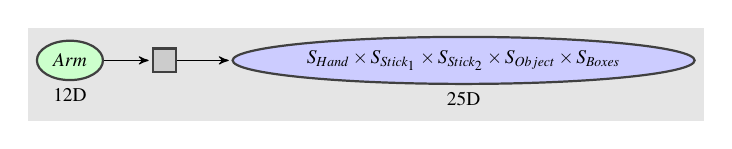
\begin{tikzpicture}[node distance=1.2cm,>=stealth',bend angle=45,auto]

	\tikzstyle{dom}   = [ellipse, thick, draw=black!75, fill=blue!20,  minimum height=4mm, minimum width=4mm]
	\tikzstyle{prim dom}   = [dom,  minimum height=5mm, minimum width=5mm,  fill=green!20]
	\tikzstyle{mod} = [rectangle, thick, draw=black!75, fill=black!20, minimum size=3mm]

	\begin{scope}[local bounding box=bb]
		\scriptsize
		\node [prim dom, label=below:$12$D] (pd1) {$Arm$};

		\node [mod] (m1) [right of=pd1] {}
		edge [pre]                  (pd1);

		\node [dom] (d1) [right of=m1, xshift=2.6cm, label=below:$25$D] {$S_{Hand} \times S_{Stick_1} \times S_{Stick_2} \times S_{Object} \times S_{Boxes}$}
		edge [pre]                (m1);
		
		
	\end{scope}
	\begin{pgfonlayer}{background}
                \node  [fill=black!10,join=round,fit=(bb)] {};
	\end{pgfonlayer}
\end{tikzpicture}

				\vspace{-0.25cm}
				
% H2
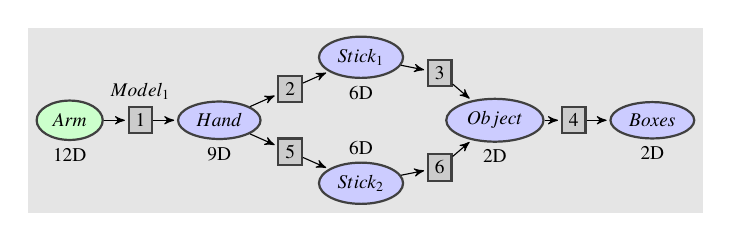
\begin{tikzpicture}[node distance=1cm,>=stealth',bend angle=45,auto]

	\tikzstyle{dom}   = [ellipse, thick, draw=black!75, fill=blue!20,  minimum height=4mm, minimum width=4mm]
	\tikzstyle{prim dom}   = [dom,  minimum height=5mm, minimum width=5mm,  fill=green!20]
	\tikzstyle{mod} = [rectangle, thick, draw=black!75, fill=black!20, minimum size=3mm]

	\begin{scope}
		\scriptsize
		\node [prim dom, label=below:$12$D] (pd1) {$Arm$};

		\node [mod, label=above:$Model_1$] (m1) [right of=pd1, xshift=-0.1cm] {$1$}
		edge [pre]                  (pd1);

		\node [dom, label=below:$9$D] (d1) [right of=m1] {$Hand$}
		edge [pre]                (m1);
		
		\node [mod] (m3) [right of=d1, xshift=-0.1cm,yshift=0.4cm] {$2$}
		edge [pre]                  (d1);
		
		\node [dom, label=below:$6$D] (d3) [right of=m3, xshift=-0.1cm,yshift=0.4cm] {$Stick_1$}
		edge [pre]                (m3);
		
		\node [mod] (m6) [right of=d1, xshift=-0.1cm,yshift=-0.4cm] {$5$}
		edge [pre]                  (d1);
		
		\node [dom, label=above:$6$D] (d6) [right of=m6, xshift=-0.1cm,yshift=-0.4cm] {$Stick_2$}
		edge [pre]                (m6);
		
		\node [mod] (m7) [right of=d6,yshift=0.2cm] {$6$}
		edge [pre]                  (d6);
		
		\node [mod] (m4) [right of=d3,yshift=-0.2cm] {$3$}
		edge [pre]                  (d3);
		
		\node [dom, label=below:$2$D] (d4) [right of=m4, xshift=-0.3cm,yshift=-0.6cm] {$Object$}
		edge [pre]                (m4)
		edge [pre]                (m7);
		
		\node [mod] (m5) [right of=d4] {$4$}
		edge [pre]                  (d4);
		
		\node [dom, label=below:$2$D] (d5) [right of=m5] {$Boxes$}
		edge [pre]                (m5);
		
		
	\end{scope}
	\begin{pgfonlayer}{background}
		\filldraw [line width=2mm,black!10]
		(d3.north  -| d5.east)  rectangle (d6.south  -| pd1.west);
	\end{pgfonlayer}
\end{tikzpicture}

				\vspace{-0.5cm}
				\caption{Architectures. Top: Flat. Bottom: Hierarchical.}
				\label{Architectures}					
			\end{figure}
				
		%
		
		\subsubsection{Hierarchical architectures}
			
			The $25$D sensory space can be structured to reflect the interaction of the different items of the environment.
			Indeed, the arm motor position influence the gripper, which influence one of the tools (but not both at the same time), which influence the position of the object and the filling of the boxes.
			We thus study here learning architectures that could make use of this sensorimotor structure, and we call them hierarchical.
			Those architecture learn $6$ models at the same time (see Fig. \ref{Architectures}: gray squares are models). 
			Each of those models functions in the same way as the random goal babbling flat architecture (F-RGB). 
			Each model has a motor space (e.g. motor space of model $2$ is $S_{Hand}$), a sensory space (respectively $S_{Stick_1}$, see arrows in Fig. \ref{Architectures}, and can choose goals randomly in this sensory space.
			At each iteration, the architecture first have to choose the model in which to choose a goal, a procedure that we call Model Babbling.
			Once a model is chosen, it finds a goal in its sensory space, and infer motor parameters (that can be in a sensory space) to reach that goal.
			Then, it passes those parameters as a goal to be reached by the lower-level model, 
			which similarly infers motor parameters and passes those ones until the actual $Arm$ motor space gets parameters to try in the environment (with the same exploration noise as in Flat architectures).
			Model $4$ have also to choose which lower-level model to use in order to reach an object end position $s_o$ in $S_{Object}$, as two models ($3$ and $6$) have $S_{Object}$ as sensory space. 
			Model $4$ chooses the tool that have allowed to reached $s_o$ as close as possible in the past.
			Finally, when motor parameters $m$ have been tested in the environment and feedback $s$ received, the mappings of all models are updated, but if model $4$ chose one tool then the mapping of the other tool is not.\\
			
		%
		
		\subsubsection{Random vs Active Model Babbling}
		
			A first condition is to randomly choose the model that will find a goal, this is Random Model Babbling (H-RMB).
			The problem of Model Babbling is an instance of strategic learning \cite{nguyen2012}, 
			where different outcomes and strategies to learn them are available and the agent learns which strategies are useful for which outcomes.
			In that paper, they show that an active choice of the outcomes and strategies based on the learning progress on each of them increase learning efficiency compared to random choice.
			To develop active learning strategies, we first define a measure of learning progress for each of the $6$ models.
			When a model has been chosen to babble, it draws a random goal $s_g$, and finds motor parameters $m$ to reach it using the lower-level models.
			The actual outcome $s$ in the sensory space of the model, associated to $m$ might be very different from $s_g$ as this goal might be unreachable, or because lower-level models are not mature enough for that goal.
			We define the competence associated to a goal $s_g$ as minus the distance between the goal and the reached point, divided by the maximal distance in this space, to scale this measure across different spaces:
			
			\begin{equation}
				C(s_g)=-\frac{||s_g-s||}{max_{s'}||s'-s||}
			\end{equation}
			 and the interest $I(s_g)$ associated to this goal as 
			\begin{equation}
				I(s_g) = |C(s_g) - mean_{kNN}C(s)|
			\end{equation}
			the absolute difference between $C(s_g)$ and the mean competence of the ($k=20$) nearest previous goals.
			The interest of a model is initialized at $0$ and updated to follow the interest of the goals (with rate $n=200$):
			\begin{equation}
				I_{model}=\frac{n-1}{n}~I_{model} + \frac{1}{n}~I(s_g)
			\end{equation}
			In condition H-P-AMB, the choice of model is proportional to their interest (probabilities are proportional to interest but with $\epsilon=10\%$ of random choice). 
			In condition H-GR-AMB, the choice of model is greedy (model with maximum interest) but also with $\epsilon=10\%$ of random choice.
			Finally, condition H-P-AMB-ATC is the same as H-P-AMB but the choice of the tool to use (model $3$ or $6$) is with probabilities proportional to the interest of the two models, 
			instead of being based on the more competent tool for the given object goal position.

		%
	
%


\section{Results}
	
	We perform $100$ simulations per condition. 
	Each simulation starts with $100$ iterations of motor babbling and then runs for $100000$ iterations of the condition.
	In this section we provide results for different types of measures. 
	First we show an exemple of a run of a hierarchical condition to illustrate a possible evolution of the interest of each model, and the result in the exploration of the object space.
	Then, we define a behavioural measure to categorize the different types of behaviours with objects and study the structure of their evolution.
	We also give a measure of the total exploration of the different spaces during simulations.
	Finally, we compare the structure of tool choice made to reach object goal position during exploration in the two conditions for which only this choice differs.
		
	Fig. \ref{res_interests} shows details about one trial of the condition H-P-AMB. 
	We can see the interest of each model during the whole experiment.
	The interests of models 2 and 5 increase abruptly once the arm succeeded in grabbing the corresponding stick.
	Following that, the interests of models 3 and 6 also increase abruptly when the object has been touched by the corresponding stick.
	An exemple of exploration of the $2$D space with the object is also provided in Fig. \ref{res_interests}(b) corresponding to the same condition.
	
	\begin{figure*}[ht]
		\centering
		\subfloat[]{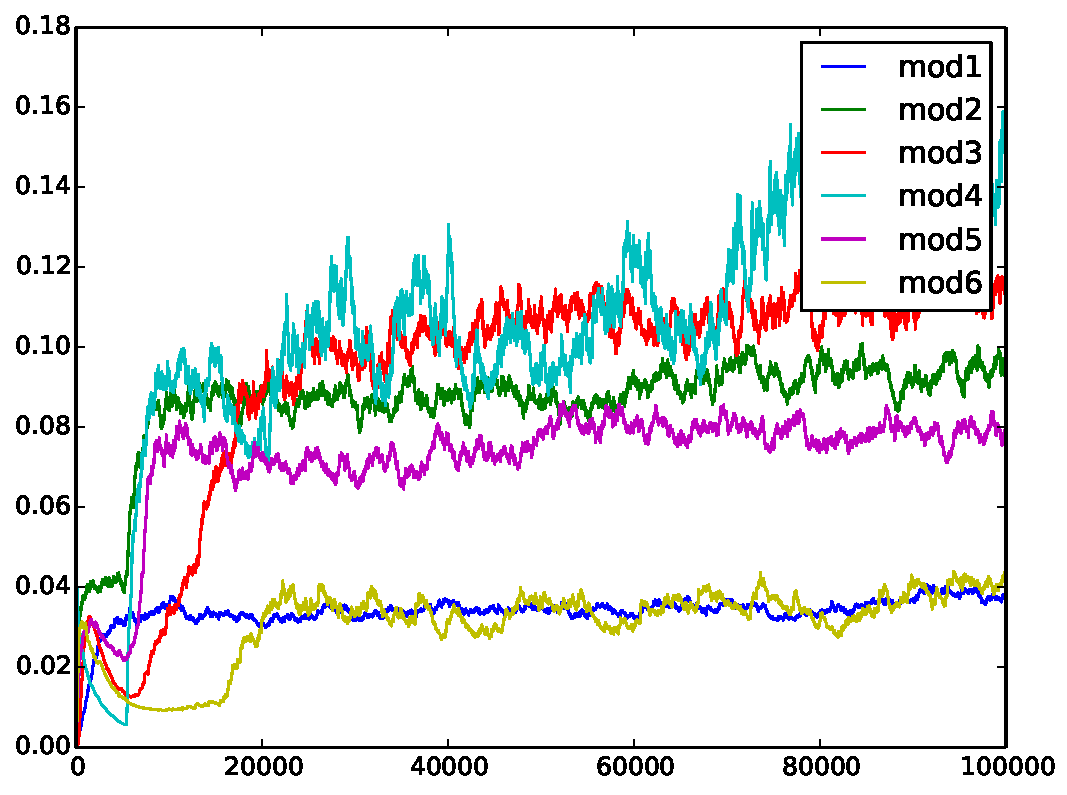
\includegraphics[width=7cm]{./include/H-RGB-P-AMB-log9-interests-100000.pdf}}
		\subfloat[]{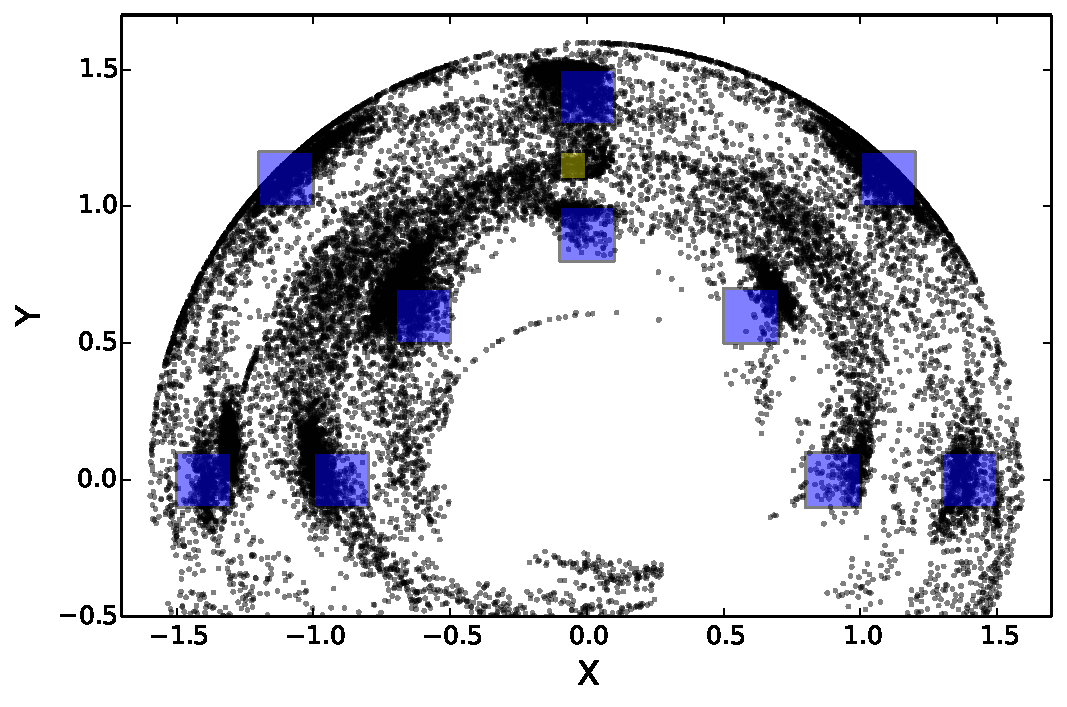
\includegraphics[width=7cm]{./include/H-RGB-P-AMB-log9-obj-explo.pdf}}
		\caption{Condition H-P-AMB. (a) Interests of each model. (b) Exploration of the object space: each dot is one point reached with the object at the end of one movement.}
		\label{res_interests}
	\end{figure*}


	
	\subsection{Structure of the evolution of behaviours}
	
		We provide a measure of the different types of behaviours with the sticks and the object during exploration. 
		We categorize the behaviours into three types.
		In the first category ($hand$) are mouvements of the arm that did not grab any stick and thus did not move the out-of-reached object.
		The second category ($stick$) are mouvements that did grab one of the two sticks but did not touch the object with it.
		The third category ($object$) contains the mouvements where both a stick was grabbed and the object was moved by the stick.
		Fig. \ref{res_ow} shows the prototypical evolution of the proportion of the three categories of behaviour along the $100000$ iterations for conditions H-GR-AMB and H-P-AMB.
		We performed a more detailed analysis by counting the trials where the evolution of the three types of behaviours were similar to the one of Fig. \ref{res_ow}(b).
		A structure was considered similar if it validated each of the following criteria:
		behaviours of categories $stick$ and $object$ increase quikly from $0$ to more than $10\%$ (potentially after an initial phase with a steady low value), 
		and are followed by a plateau (steady curve with small slope) with no abrupt changes, and behaviours of category $object$ start to raise at least $1000$ iterations after $stick$ started to raise.
		See Table \ref{table} for the results of this analysis per condition.
		Also, the median number of abrupt changes across trials for each condition are reported in the same table (as the sum of steady changes of more than $10\%$ in the three behaviours).
		with a significant difference between condition H-GR-AMB and the others (Mann-Whitney U tests, $p<0.0001$).

		\begin{table}[!ht]
			\small
			\begin{center} 
			\caption{behavioural analysis} 
			\label{table} 
			\vskip 0.12in
			\begin{tabular}{| c | c | c |} 
				\hline
				Condition  &  \begin{tabular}{@{}c@{}}Number of Trials \\ validating criteria\end{tabular}   & \begin{tabular}{@{}c@{}}Median number of  \\ Abrupt changes \end{tabular}\\
				\hline
				F-RmB        &    0 &  0\\
				F-RGB        &    0 &  1\\
				H-RMB        &   60 &  2\\
				H-P-AMB      &   70 &  2\\
				H-GR-AMB     &    7 &  6\\
				H-P-AMB-ATC  &   79 &  1\\
				\hline
			\end{tabular} 
			\end{center} 
		\end{table}

		\begin{figure}[ht]
			\centering
			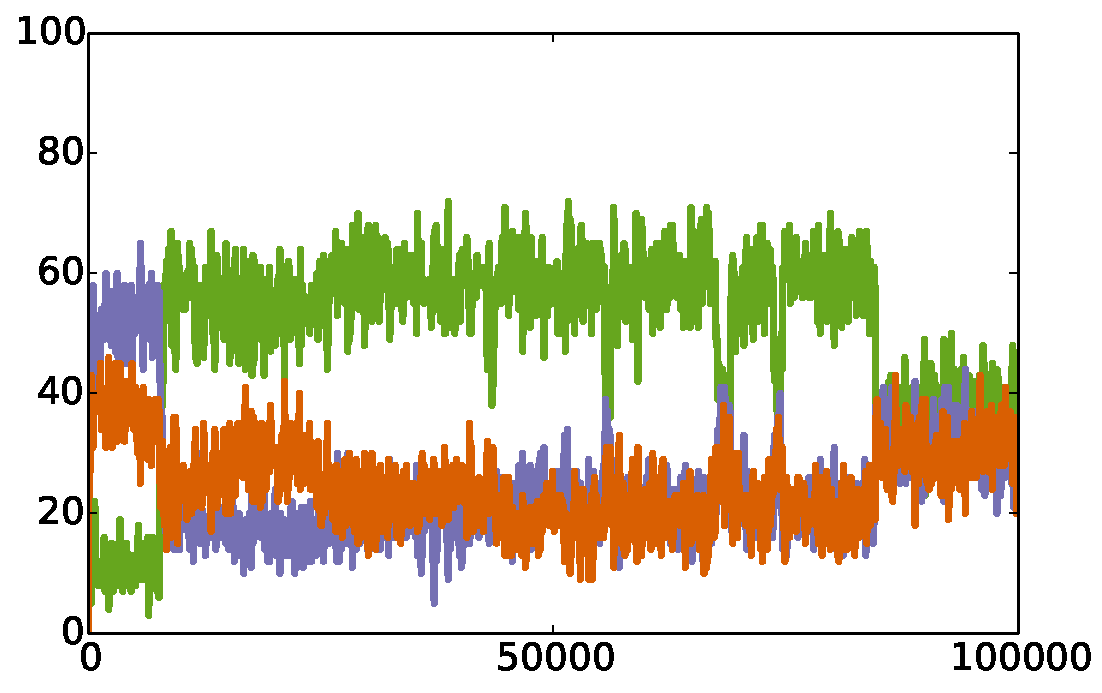
\includegraphics[width=4.4cm]{./include/H-RGB-GR-AMB-log15-events-100000.pdf}
			\hspace{-0.4cm}
			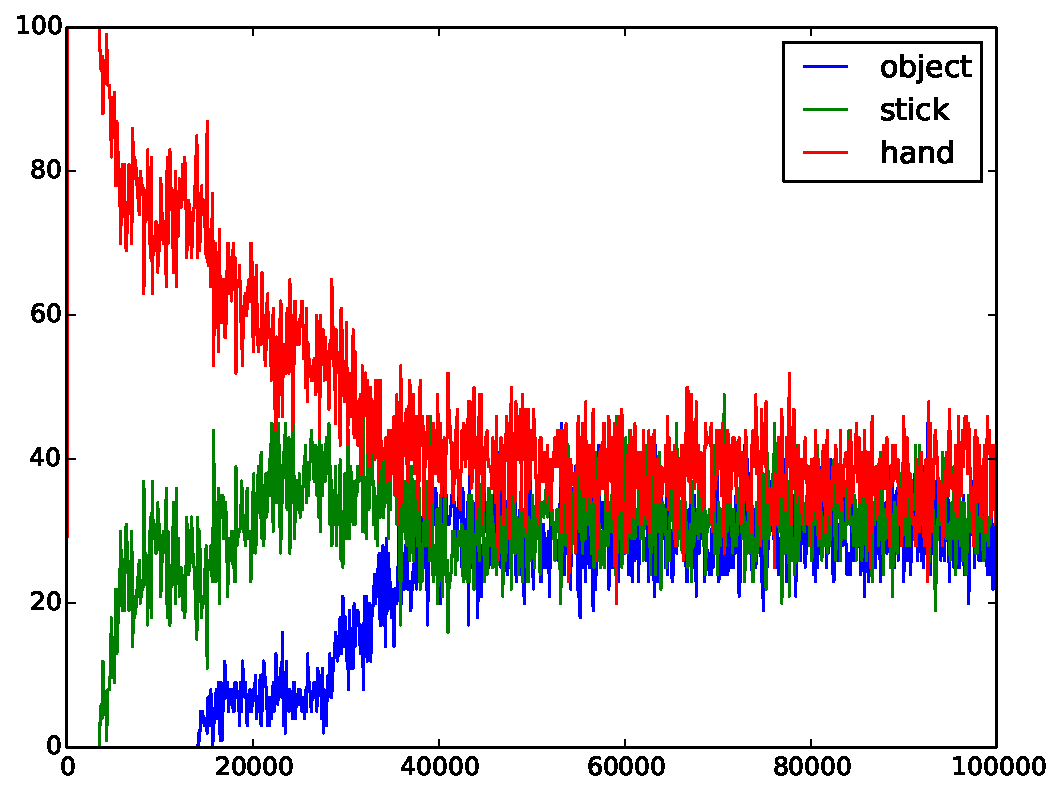
\includegraphics[width=4.4cm]{./include/H-RGB-P-AMB-log8-events-100000.pdf}
			\caption{behavioural measure. Left: H-GR-AMB, Right: H-P-AMB.}
			\label{res_ow}
		\end{figure}
		
	%
	
	
	\subsection{Exploration efficiency}

		Also, for each condition we measure the total exploration of the different sensory spaces during training. 
		The exploration of the hand, sticks and object spaces is defined as the number of reached cells 
		in a $100\times100$ discretization of the (X,Y) space of the position at timestep $50$ (end of movement).
		The exploration of the boxes is the number of boxes that have been filled with the object during training.
		Fig. \ref{res_explo} shows the total exploration of the different sensory spaces for each condition.
		We provide statistical Mann-Whitney U test results of comparisons of the exploration in different pairs of conditions.
		Firstly, the Motor Babbling condition (F-RmB) have more explored $S_{Hand}$ and less $S_{Object}$ and $S_{Boxes}$ compared to the other conditions ($p<0.0001$).
		Then, F-RGB explores all spaces less than H-RMB condition ($p<0.01$).
		H-RMB explores more $S_{Hand}$ ($p<0.001$) and less $S_{Object}$ ($p<0.05$) than H-P-AMB.
		Also, H-GR-AMB shows lower exploration all spaces than H-P-AMB ($p<0.01$).
		Condition H-P-AMB-ATC explores more $S_{Stick_2}$ ($p<0.05$) than condition H-P-AMB, and difference is not significant in other spaces.
		
		\begin{figure*}[ht]
			\centering
			
\includegraphics[width=14cm]{./include/xp1-explo-legend.pdf}\\
			\vspace{-0.4cm}
			\subfloat[$Hand$]{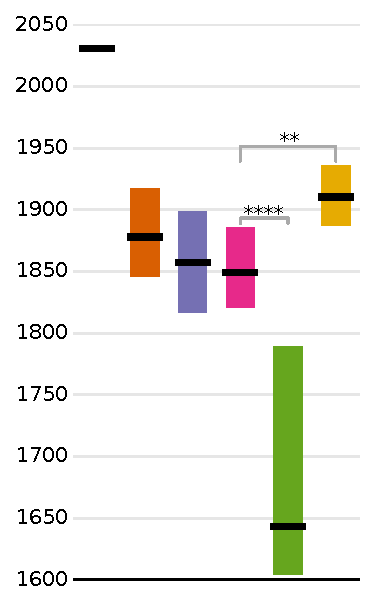
\includegraphics[width=3.5cm]{./include/xp1-explo-hand.pdf}}
			\subfloat[$Stick_1$]{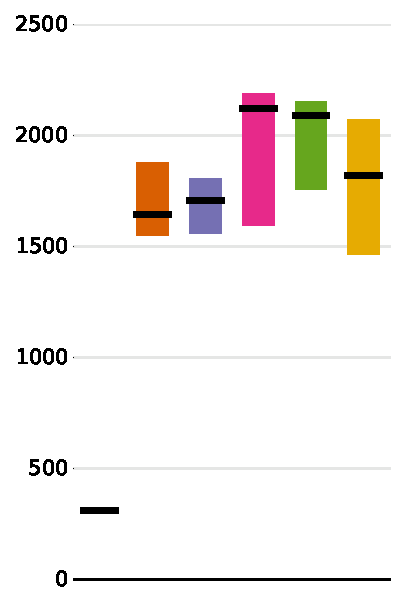
\includegraphics[width=3.5cm]{./include/xp1-explo-stick_1.pdf}}
			\subfloat[$Stick_2$]{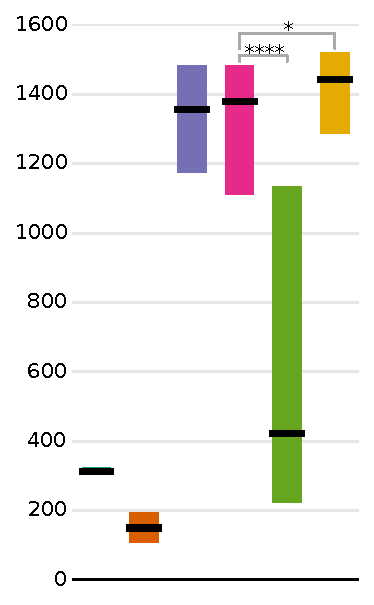
\includegraphics[width=3.5cm]{./include/xp1-explo-stick_2.pdf}}
			\subfloat[$Object$]{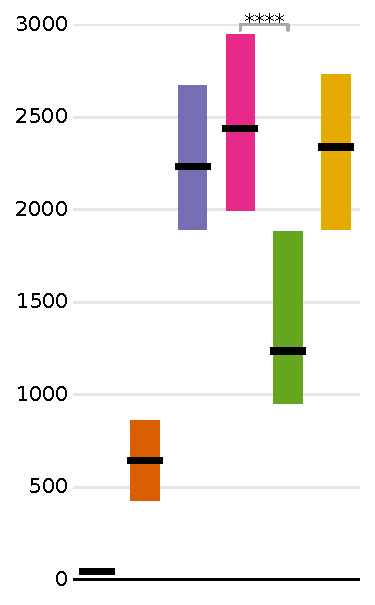
\includegraphics[width=3.5cm]{./include/xp1-explo-obj.pdf}}
			\subfloat[$Boxes$]{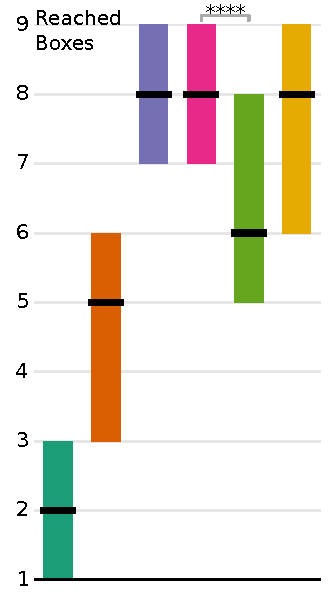
\includegraphics[width=3.3cm]{./include/xp1-explo-box.pdf}}
			\caption{Exploration of sensory spaces. Box plots show for each condition and space the median and quartiles of the $100$ trials.}
			\label{res_explo}
		\end{figure*}

	%
	
	\subsection{Structure of tool choice}

		Fig. \ref{res_choice} shows a comparison of the choice of tool to reach a given object goal position in the conditions H-P-AMB and H-P-AMB-ATC.
		In those conditions, model $4$ learns a mapping between $S_{Object}$ and $S_{Boxes}$. 
		When this model is babbling, it chooses a random goal $s_b \in S_{Boxes}$ and infers the best object position $s_o$ to reach $s_b$.
		To reach $s_o$, one of the tools ($Stick_1$ with model $3$ or $Stick_2$ with model $6$) is chosen. 
		We plot all those choices model $4$ made during exploration, at position $s_o$ on a $2$D space, with color blue if $Stick_1$ was chosen and red if $Stick_2$ was chosen, in one figure for each of the two conditions.
		We can see two very different choice structures.
		However, goal that can be reached with both tools are more often chosen to be explored with the long stick in the interest-based choice of condition H-P-AMB-ATC than in competence-based choice of condition H-P-AMB.
		
		\begin{figure}[ht]
			\centering
			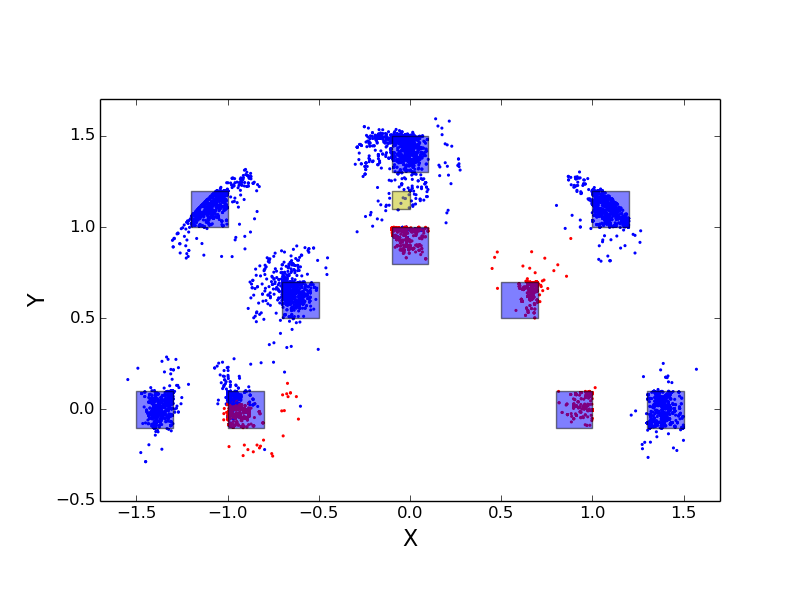
\includegraphics[width=4.5cm]{./include/H-RGB-P-AMB-log9-choice_mod4.png}
			\hspace{-0.6cm}
			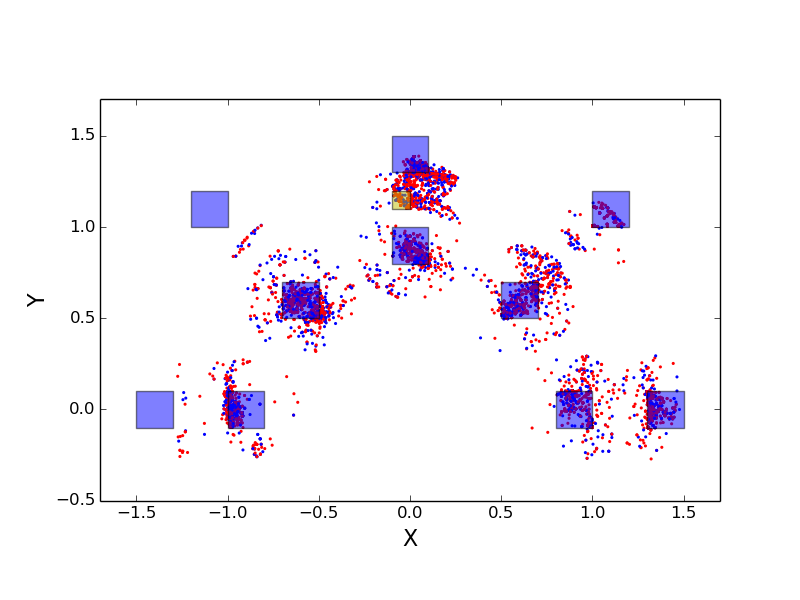
\includegraphics[width=4.5cm]{./include/H-RGB-P-AMB-PGITC-log3-choice_mod4.png}
			\caption{Chosen tool depending on object goal position. Blue points: long stick choice. Red points: small stick choice. Left: H-P-AMB, Right: H-P-AMB-ATC.}
			\label{res_choice}
		\end{figure}
		
	%
	
%


\section{Discussion}

	\subsection{Structure of the evolution of behaviours}
	
		Results show different structures of behaviour evolution in the different conditions.
		H-GR-AMB shows successive behavioural steps with abrupt changes.
		Random model babbling and active model babbling both show overlapping waves structure in the evolution of the three behaviours, 
		but random model babbling explores slightly less the object position.
		In this setup, the difference is more on the cognitive or intentional level, as active model babbling monitors the progress on each model whereas random model babbling do not, than on a quantitative level, 
		because here all models are still useful to explore.
		However, in others setups where some tasks are learned much faster than others and where at some point it become useless to explore a mastered task, then active model babbling would
		make a key difference on a quantitative exploration point of view, and on the structure of the evolution of the measured behaviours.
	
	%
	
	\subsection{Variability of strategies to reach goals}
	
		Different structure of tool choice: overlapping waves of strategies to fulfill given goals in condition H-P-AMB-ATC.
	
	%
	
%




\bibliographystyle{apacite}

\setlength{\bibleftmargin}{.125in}
\setlength{\bibindent}{-\bibleftmargin}

\bibliography{include/bibliography}


\end{document}
